\chapter{ПРОЕКТИРОВАНИЕ И ТЕСТИРОВАНИЕ ГЕНЕРАТОРА СИГНАЛОВ}
\section{Проектирование генератора сигналов}
	По структурной схеме (рис. 2.7) создадим фрагмент схемы электрической принципиальной. 
	
	\begin{figure}[H]
    \centering
    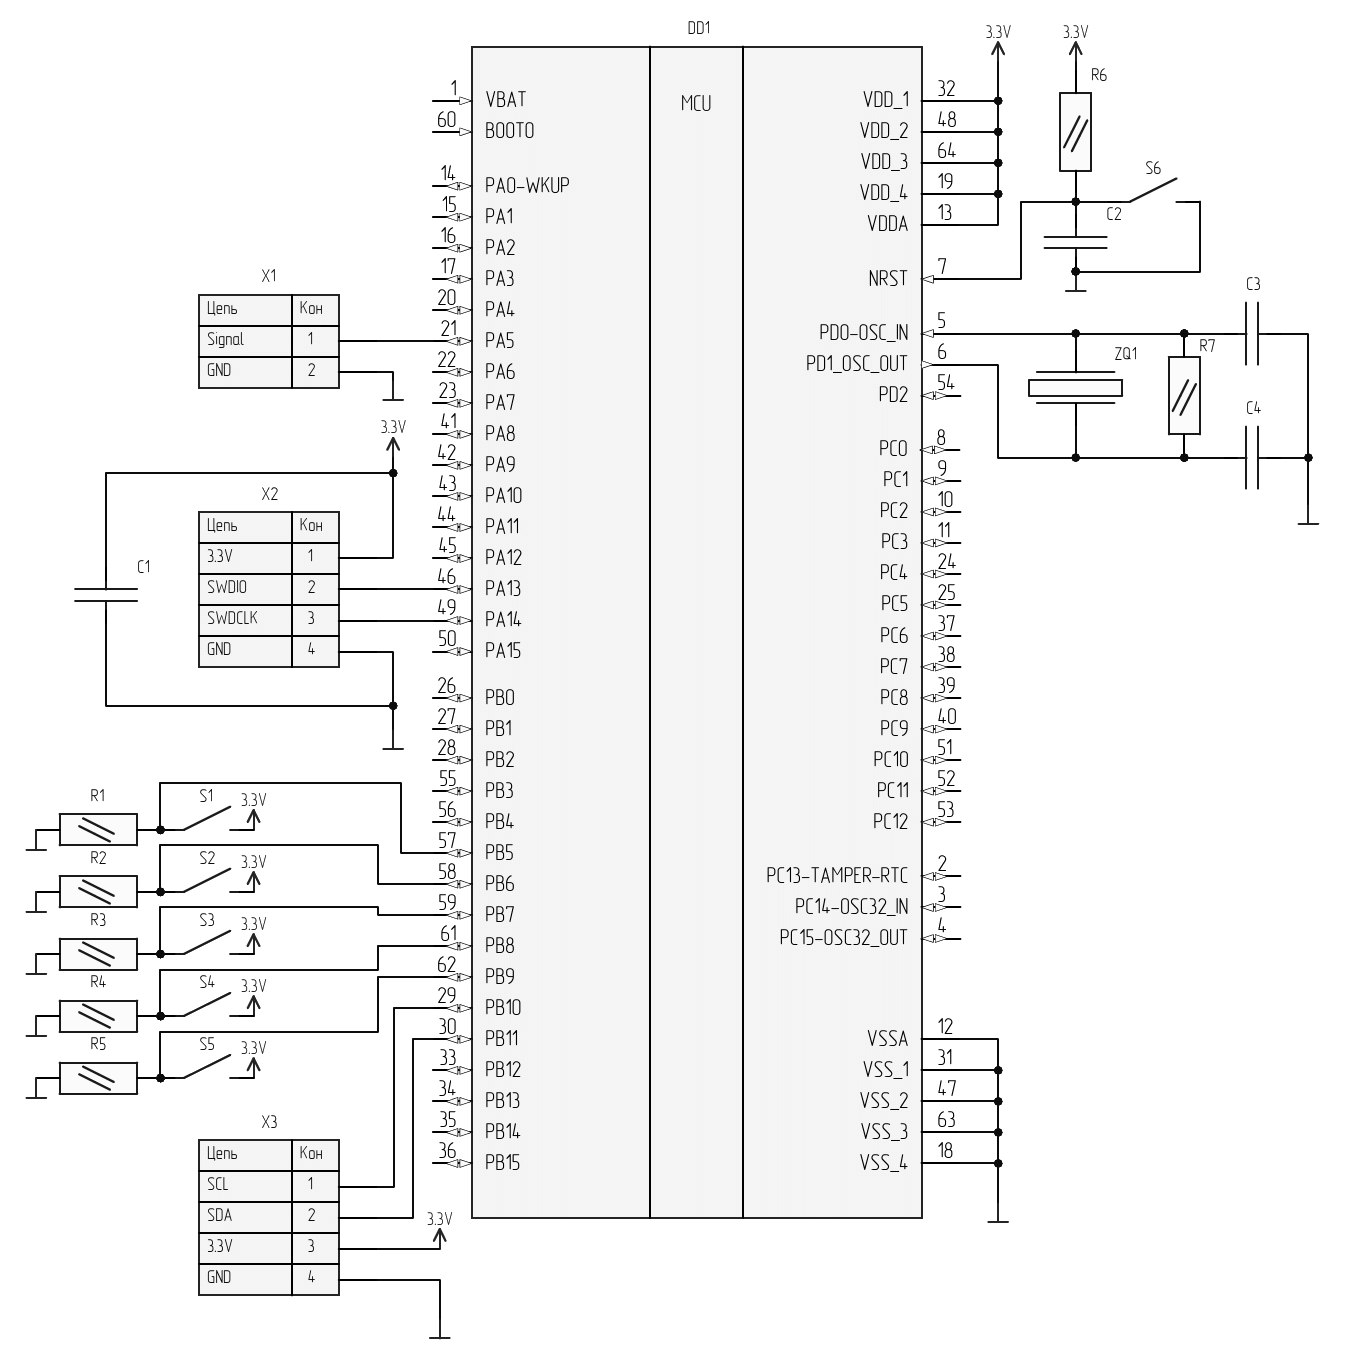
\includegraphics[width=1\textwidth]{../image/scheme-cropped.png}
    \caption{Фрагмент схемы электрической принципиальной.}
	\end{figure}
	
	Просто так контроллер работать не сможет. Необходим внешний кварцевый резонатор для стабилизации частоты системного тактового генератора, а также функция сброса. Эти узлы уже реализованы на отладочной плате микроконтроллера. Питание схемы будет подаваться через разъём SWD.
		
	Для улучшения генерации будет задействован встроенный в цифро-аналоговый преобразователь выходной буфер. При его использовании он будет срезать сигнал сверху и снизу на 0.2В, поэтому значения тоже следует срезать на эту же величину для корректной генерации.
	
	В документе от STM про работу с цифро-аналоговым преобразователем есть формула для расчета выходного напряжения~\cite{an3126}.
	
	\begin{gather}
	DAC_{output} = V_{REF}*\dfrac{DOR}{DAC_{MaxDigitalValue} + 1},
	\end{gather}
	
	где $DAC_{output}$ --- выходное напряжение ЦАП,
	
	$V_{REF}$ --- опорное напряжение,
	
	$DOR$ --- цифровое значение выходного напряжения,
	
	$DAC_{MaxDigitalValue}$ --- максимальное значение $DOR$.
	
	Нам нужно найти какое значение соответствует напряжению 0.2В. Выразим DOR и подставим имеющиеся значения.
	
	\begin{center}
	$DOR = \dfrac{V_{REF}}{DAC_{output}}*DAC_{MaxDigitalValue} + 1 = \dfrac{3.3}{0.2}*(4095+1) = 248.$
	\end{center}
	
	Поэтому для отсчётов нужно будет указать смещение от нуля 248, а максимальное значение 4095 меньше на 248, то есть 3847. 
	
	Для управления установлены 5 кнопок, для которых выделены выводы PB5 - PB9. Постоянно быть подключенными к напряжению или земле выводы не могут, т. к. не будет возможности подавать на них какой-либо информационный сигнал. На выводы могут наводиться произвольные потенциалы, что негативно влияет на работу схемы. Подобные потенциалы имитируют сигналы, которые не предусмотрены. Из-за них может нарушиться логика работы, поэтому их принято фиксировать~\cite{schemat}. 
	
	Для этого используют подтягивающие (Pull - up) или заземляющие (Pull - down) резисторы. Они создают цепь, которая обеспечивает подтяжку сигнала к напряжению питания или земле. Если резисторы имеют большие сопротивления, то сигналы относят к слабым. При подключении сильных информационных сигналов происходит преодоление слабых и функциональность схемы не нарушается~\cite{butres}.
	
	\begin{figure}[H]
    \centering
    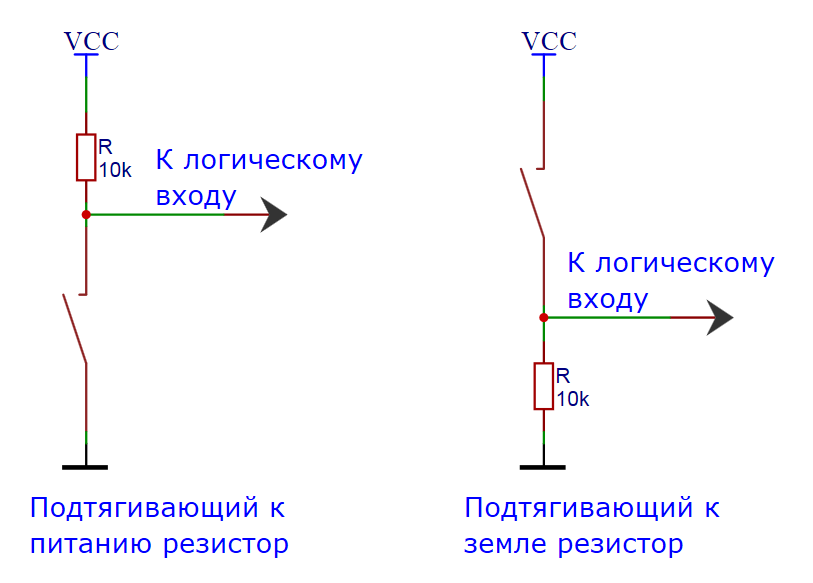
\includegraphics[width=0.55\textwidth]{../image/res.png}
    \caption{Pull-up и Pull - down резисторы.}
	\end{figure}
	
	В схеме устройства будет использоваться подтяжка к земле для считывания высокого уровня сигнала, то есть будет использоваться прямая логика. Рассчитаем минимальное и максимальное сопротивление заземляющего резистора.
	\begin{gather}
	R_{min} = \dfrac{V_{0}}{I_{max}},
	\end{gather}
	
	где $V_{0}$ --- напряжение логического нуля,
	
	$I_{max}$ --- максимальный ток вывода.
	
	Согласно спецификации микроконтроллера напряжение логического нуля составляет 1,16 В, а максимальный протекающий ток через пин может быть 25 мА~\cite{f103}. 
	
\begin{center}
	$R_{min} = \dfrac{1,16}{25*10^{-3}} = 46,4$ Ом.
\end{center}

	Для расчета максимального сопротивления формула следующая:
	\begin{gather}
	R_{max} = \dfrac{t}{C_{I/O}},
	\end{gather}
	
	где $t$ --- время нарастания сигнала,
	
	$C_{I/O}$ --- ёмкость вывода.
	
	Ёмкость вывода составляет 5 пФ, время нарастания возьмём 1 микросекунду (стандартный сигнал 100 кГц).
	
\begin{center}
	$R_{max} = \dfrac{1*10^{-6}}{5*10^{-12}} = 200$ кОм.
\end{center}	

	Из расчётов можно сделать вывод, что номинал резистора расположен в следующих границах.
	
\begin{center}
	$46,4$ Ом$ < R < 200$ кОм.
\end{center}	

	Разброс довольно большой, но из практики известно, что подтягивающий резистор имеет номинал 1 - 10 кОм.
	
	Для линий I2C также используются подтягивающие резисторы, которые уже установлены на дисплее.
	
	\begin{figure}[H]
    \centering
    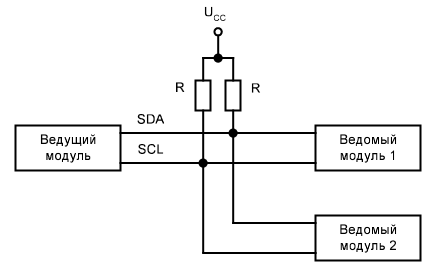
\includegraphics[width=0.525\textwidth]{../image/i2c.png}
    \caption{Организация интерфейса.}
	\end{figure}
	
	Интерфейс в микроконтроллере расположен на выводах PB10 (SCL) и PB11 (SDA). Также для дисплея потребуется питание 3.3 В.
	
	Дисплей и кнопки расположим на макетной плате размером 50 на 50 мм.
	
	\begin{figure}[H]
    \centering
    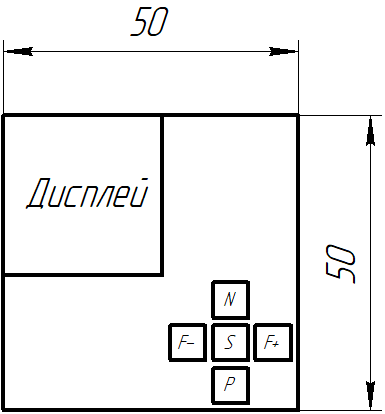
\includegraphics[width=0.45\textwidth]{../image/func_gen.png}
    \caption{Схема расположения периферии.}
	\end{figure}
	
	Назначения кнопок:
	\begin{enumerate}
	\item F- --- уменьшить частоту;
	\item F+ --- увеличить частоту;
	\item P --- предыдущий сигнал;
	\item N --- следующий сигнал;
	\item S --- переключить шаг по частоте.
	\end{enumerate}
	
	В результате сборки получилась плата с периферией.

	\begin{figure}[H]
    \centering
    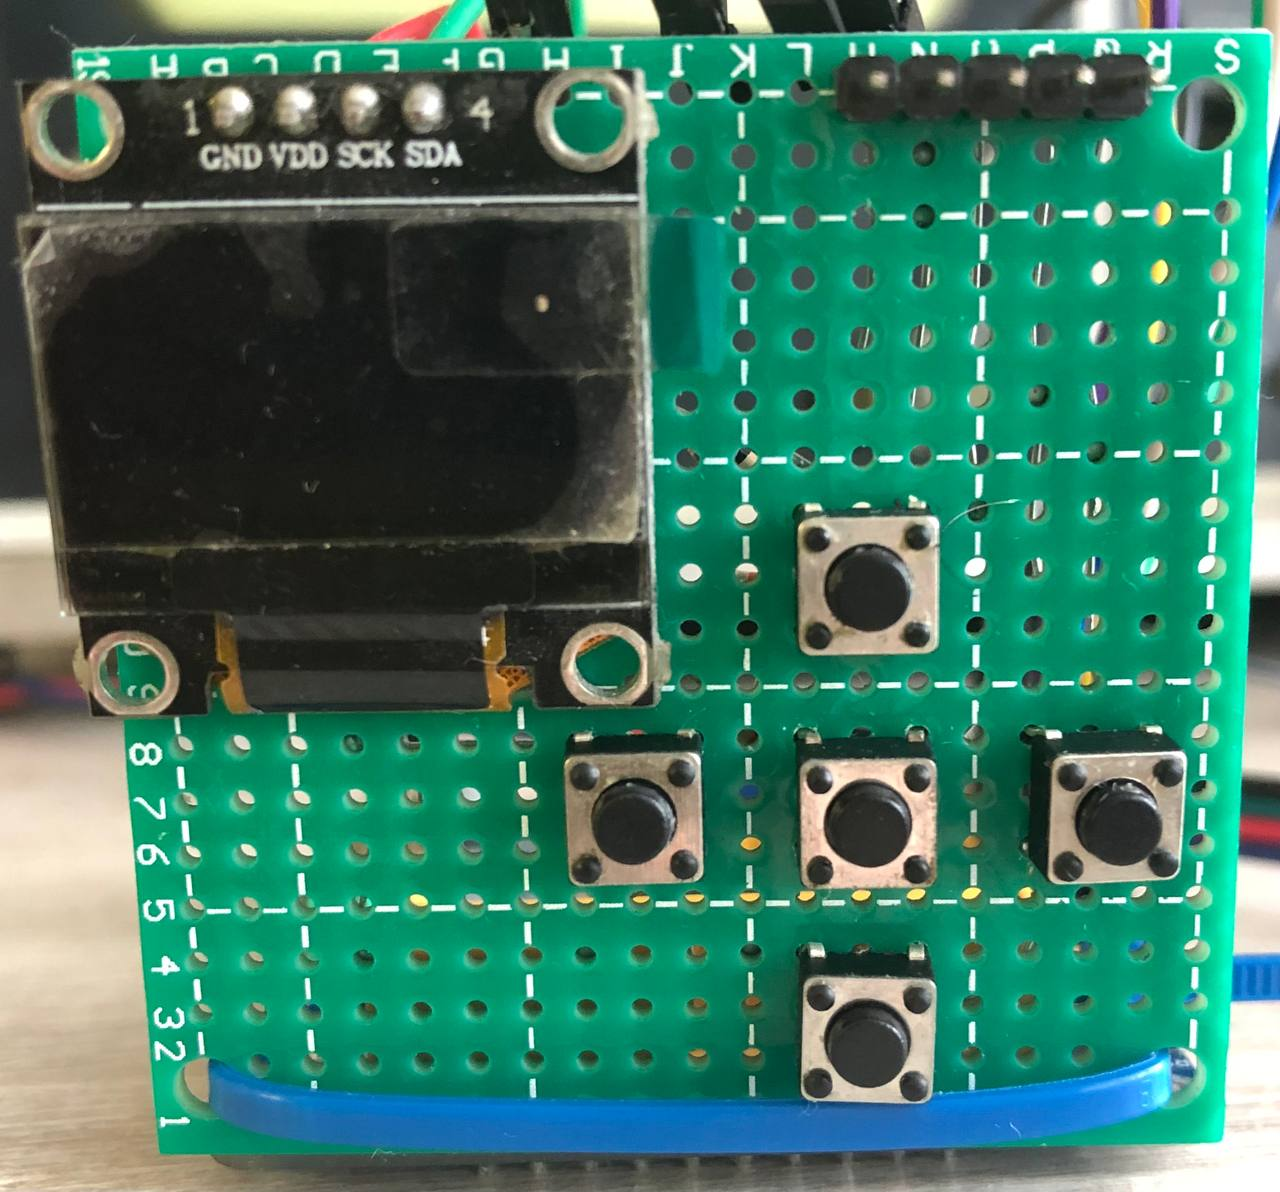
\includegraphics[width=0.5\textwidth]{../image/m1.jpeg}
    \caption{Плата периферии.}
	\end{figure}	
	
	Макет устройства будет состоять из отладочной платы микроконтроллера и полученной платы периферии. Обе части будут соединены проводами. Выход цифро-аналогового преобразователя, на котором генерируется сигнал, расположен на отладочной плате. В результате конструирования получился следующий макет устройства (рис. 3.6).

	\begin{figure}[H]
    \centering
    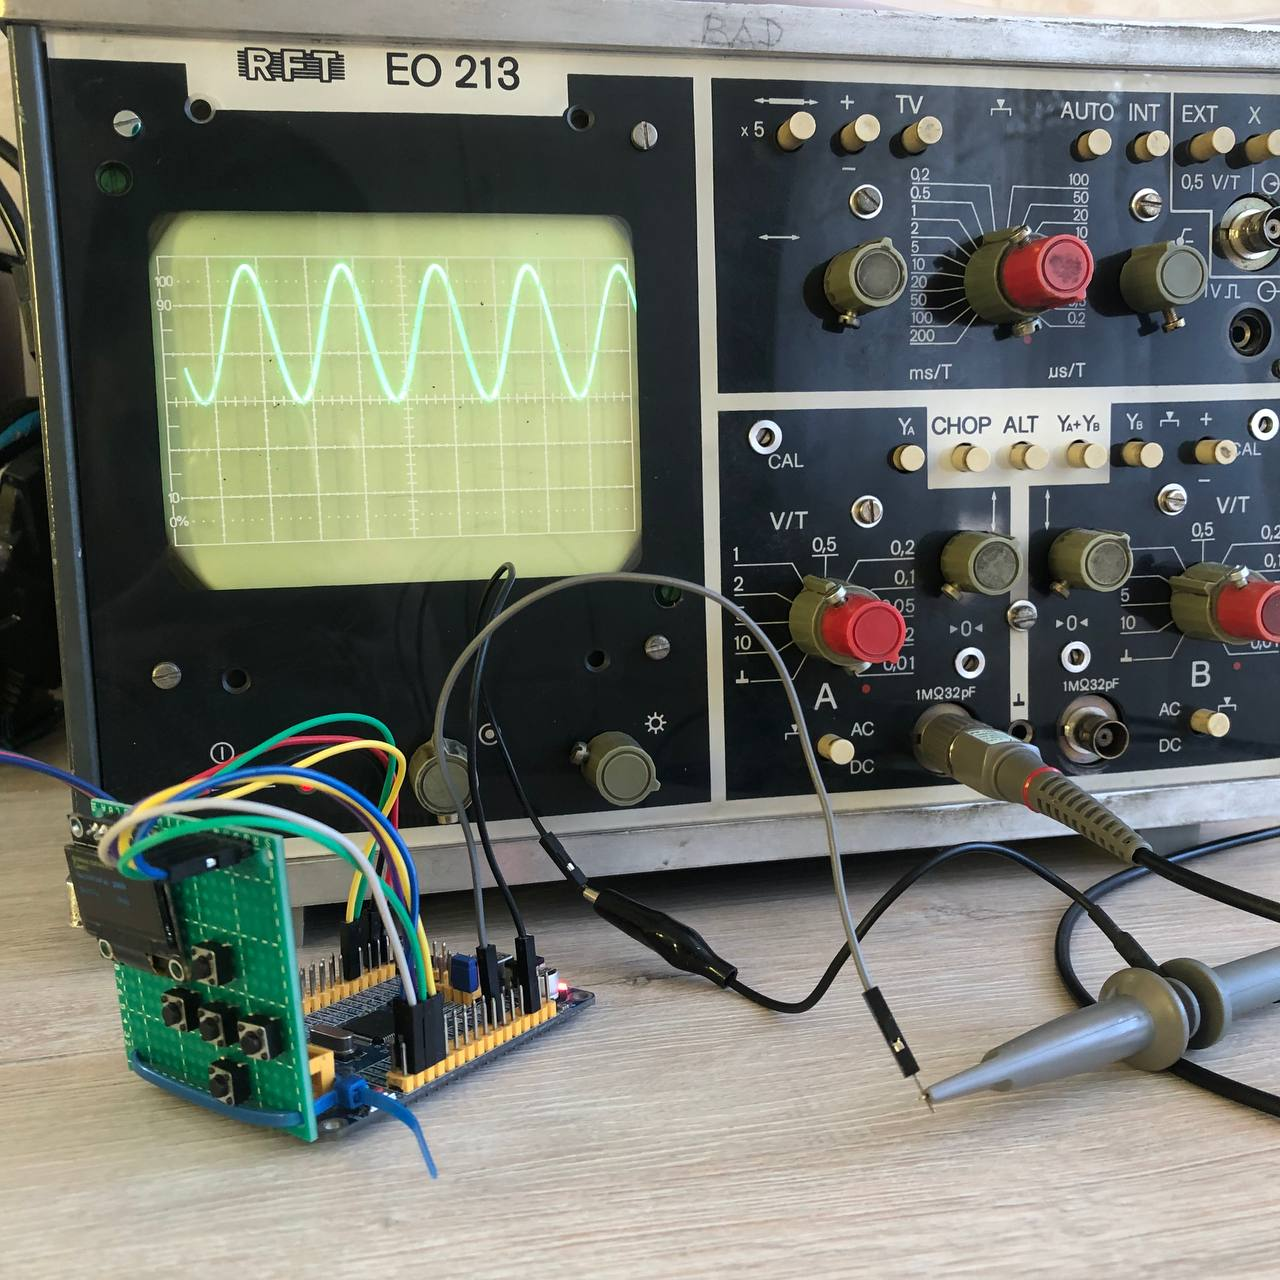
\includegraphics[width=0.5\textwidth]{../image/m2.jpg}
    \caption{Макет устройства.}
	\end{figure}	

\section{Тестирование генератора сигналов}
	
	Протестируем работоспособность полученного устройства. Будем отслеживать состояние устройства и информацию в отладчике. В отладчике будем отслеживать следующие переменные:
	\begin{itemize}
	\item f --- расчетная частота;
	\item step --- код частоты (шаг по частоте);
	\item num\_step --- номер шага;
	\item num\_sig --- номер сигнала;
	\item signal --- буфер сигнала.
	\end{itemize}		
	
	После запуска устройства на экране появляются строки с пустыми параметрами формы сигнала, частоты и шага (рис. 3.7). 

	\begin{figure}[H]\captionsetup[subfigure]{font=normalsize}
     \begin{subfigure}[H]{0.5\textwidth}
         \centering
         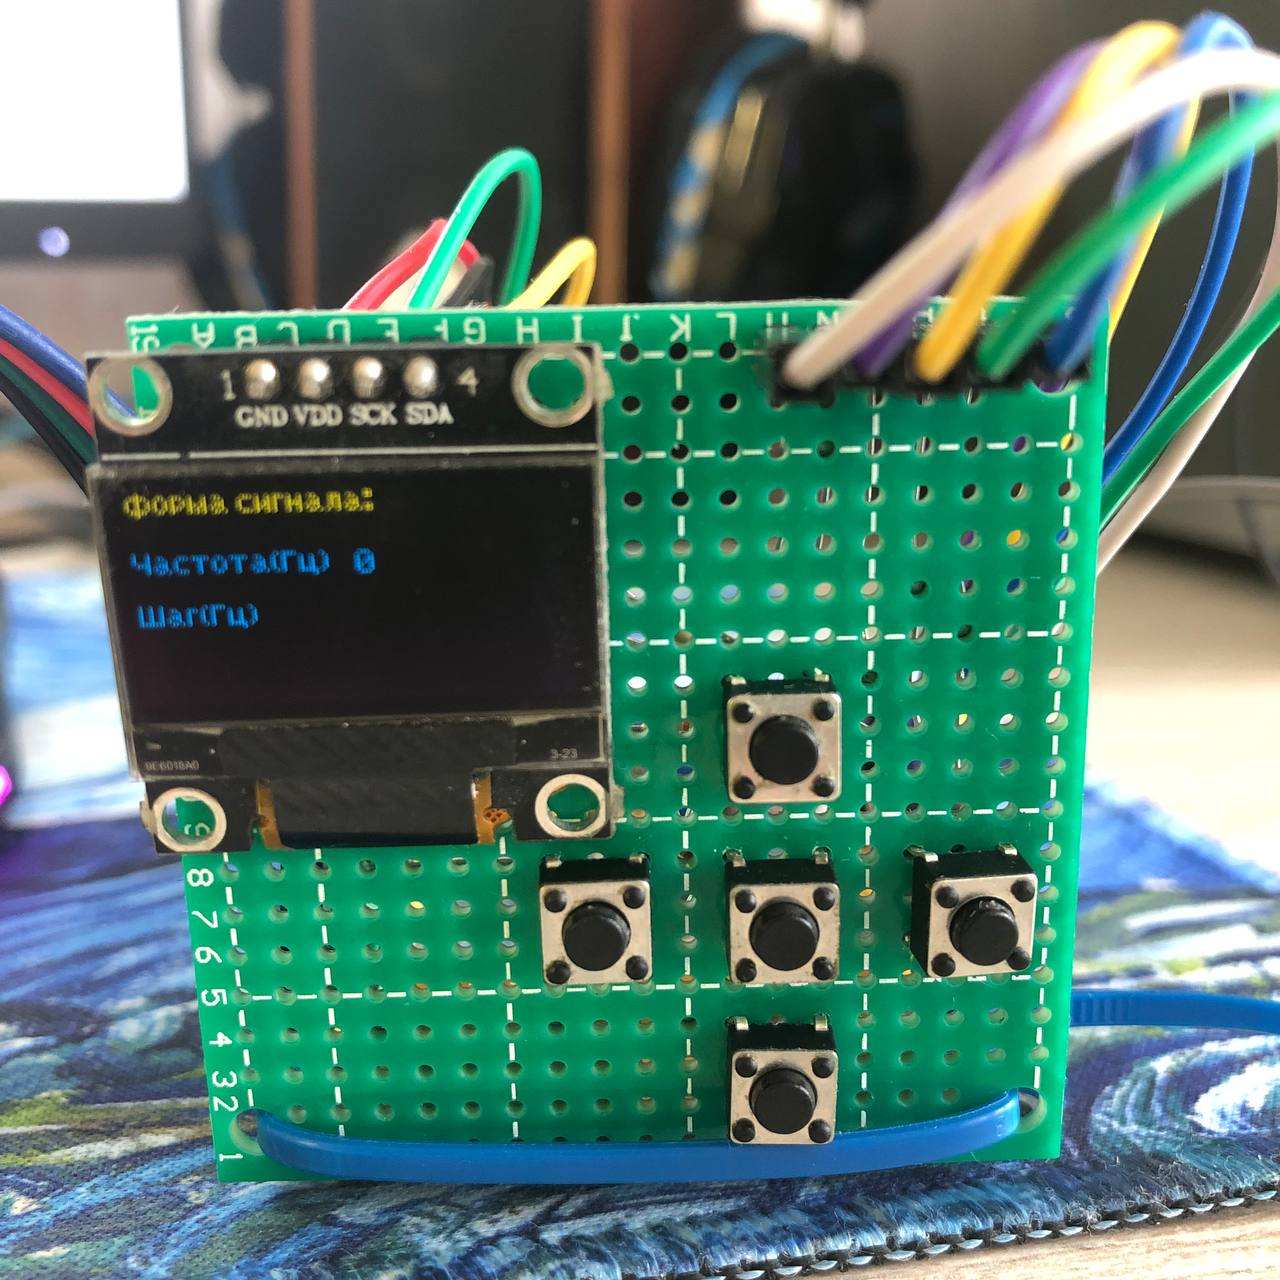
\includegraphics[width=0.6\textwidth]{../image/test0_u_s.jpg}
         \caption{Состояние устройства.}
     \end{subfigure}
     \hfill
     \begin{subfigure}[H]{0.5\textwidth}
         \centering
         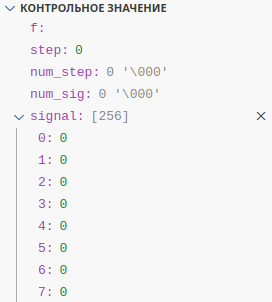
\includegraphics[width=0.525\textwidth]{../image/test0_o_s.png}
         \caption{Состояние в отладчике.}
     \end{subfigure}
        \caption{Начальное состояние устройства при запуске.}
	\end{figure}
	
	Логика работы дисплея описана блок-схемой (рис. 3.8).
	
	\begin{figure}[H]
    \centering
    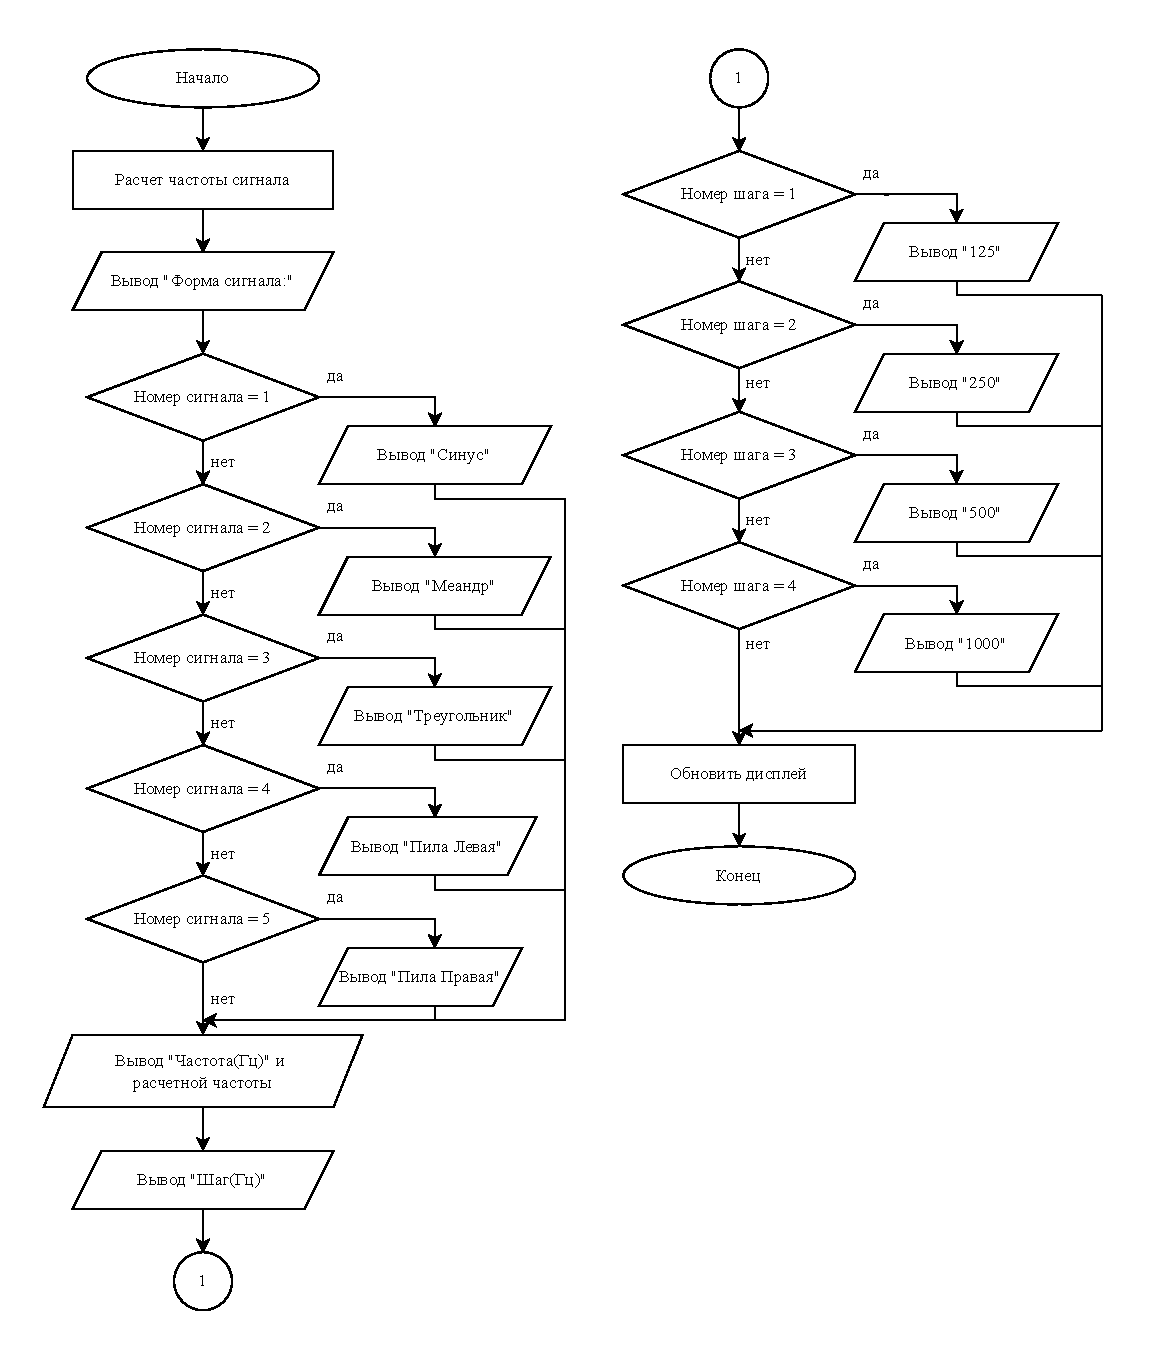
\includegraphics[width=0.775\textwidth]{../image/display.pdf}
    \caption{Блок-схема алгоритма работы дисплея.}
	\end{figure}	
	
	Требуется выставить параметры сигнала. Клавишами N и P выбирается форма сигнала. При нажатии клавиши N выполняется алгоритм, описанный блок-схемой (рис. 3.10). Для клавиши P алгоритм отличается только тем, что номер сигнала нужно декрементировать.
	
	\begin{figure}[H]
    \centering
    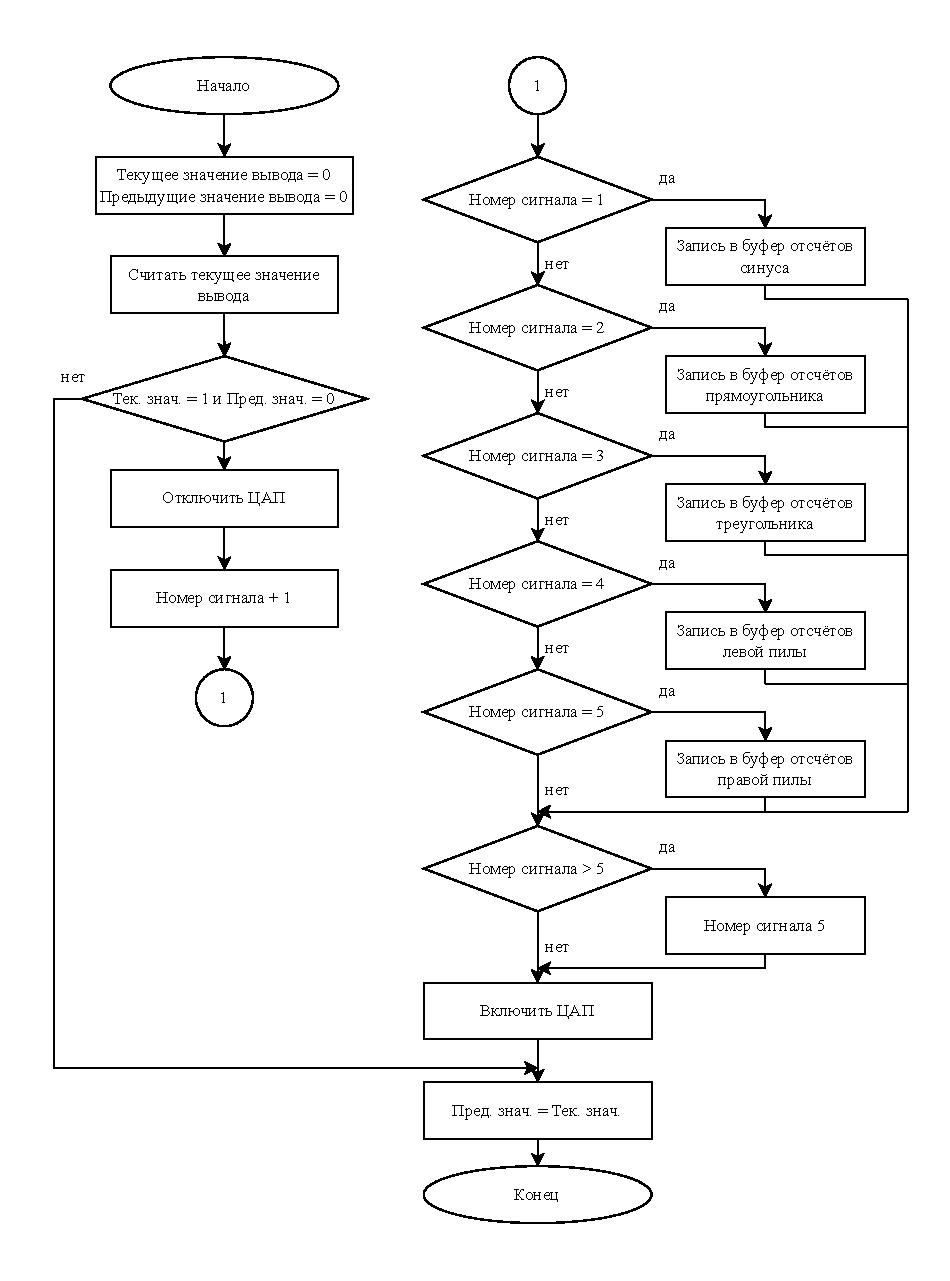
\includegraphics[width=0.8\textwidth]{../image/plus_signal.pdf}
    \caption{Блок-схема алгоритма выбора следующего сигнала.}
	\end{figure}	
	
	При выборе сигнала пользователь листает формы сигнала, а микроконтроллер заполняет буфер отсчётами выбранного сигнала. Выберем сигнал синуса.
	\begin{figure}[H]\captionsetup[subfigure]{font=normalsize}
     \begin{subfigure}[H]{0.5\textwidth}
         \centering
         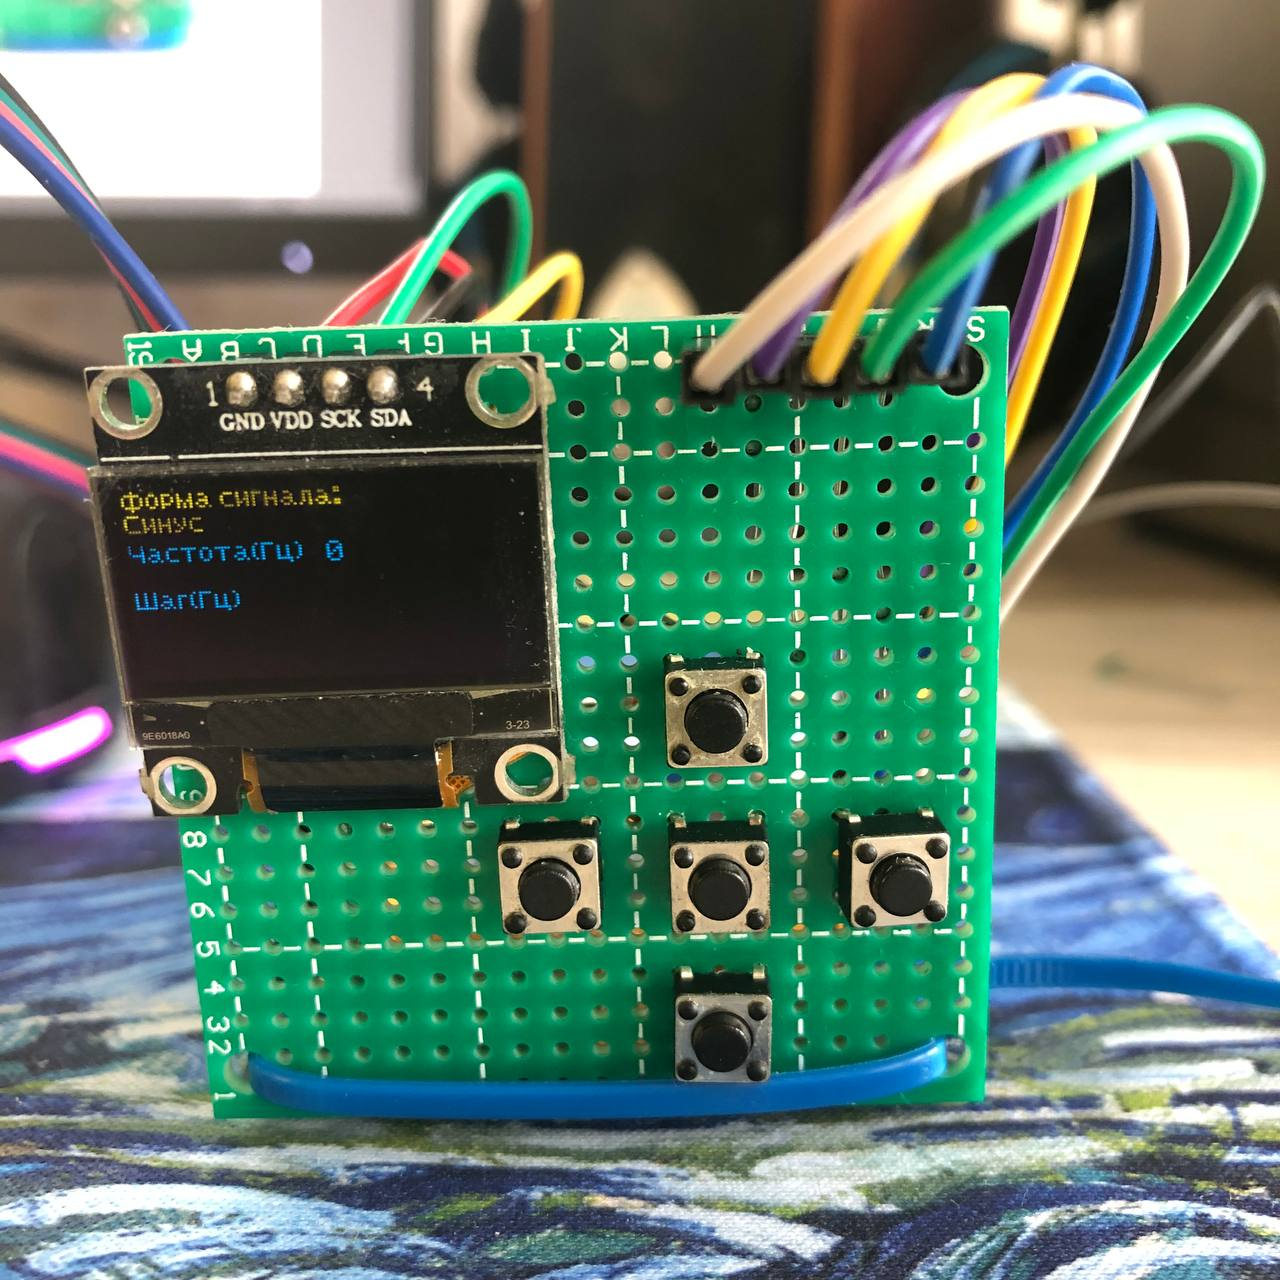
\includegraphics[width=0.6\textwidth]{../image/test1_u_s.jpg}
         \caption{Состояние устройства.}
     \end{subfigure}
     \hfill
     \begin{subfigure}[H]{0.5\textwidth}
         \centering
         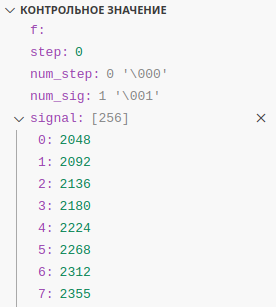
\includegraphics[width=0.525\textwidth]{../image/test1_o_s.png}
         \caption{Состояние в отладчике.}
     \end{subfigure}
        \caption{Процедура выбора синусоидального сигнала.}
	\end{figure}

	Теперь нужно выбрать величину шага, с которым будет регулироваться частота сигнала. Алгоритм для установки шага следующий (рис. 3.16).
	
	\begin{figure}[H]
    \centering
    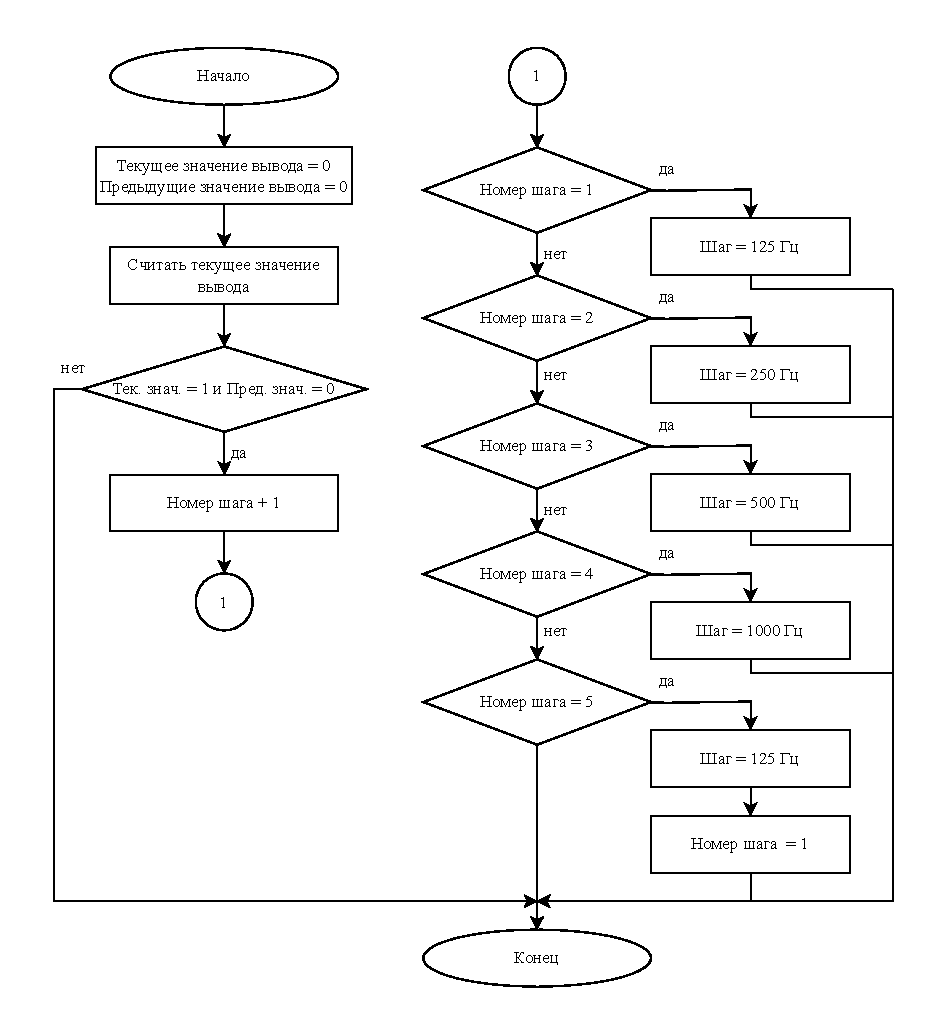
\includegraphics[width=0.8\textwidth]{../image/step_select.pdf}
    \caption{Блок-схема алгоритма выбора шага.}
	\end{figure}	
	
	Как можно заметить из блок-схемы всего есть 4 шага:
	\begin{enumerate}
		\item 125 Гц;
		\item 250 Гц;
		\item 500 Гц;
		\item 1000 Гц.
	\end{enumerate}
	
	Выберем для примера шаг 125 Гц.
	
	\begin{figure}[H]\captionsetup[subfigure]{font=normalsize}
     \begin{subfigure}[H]{0.5\textwidth}
         \centering
         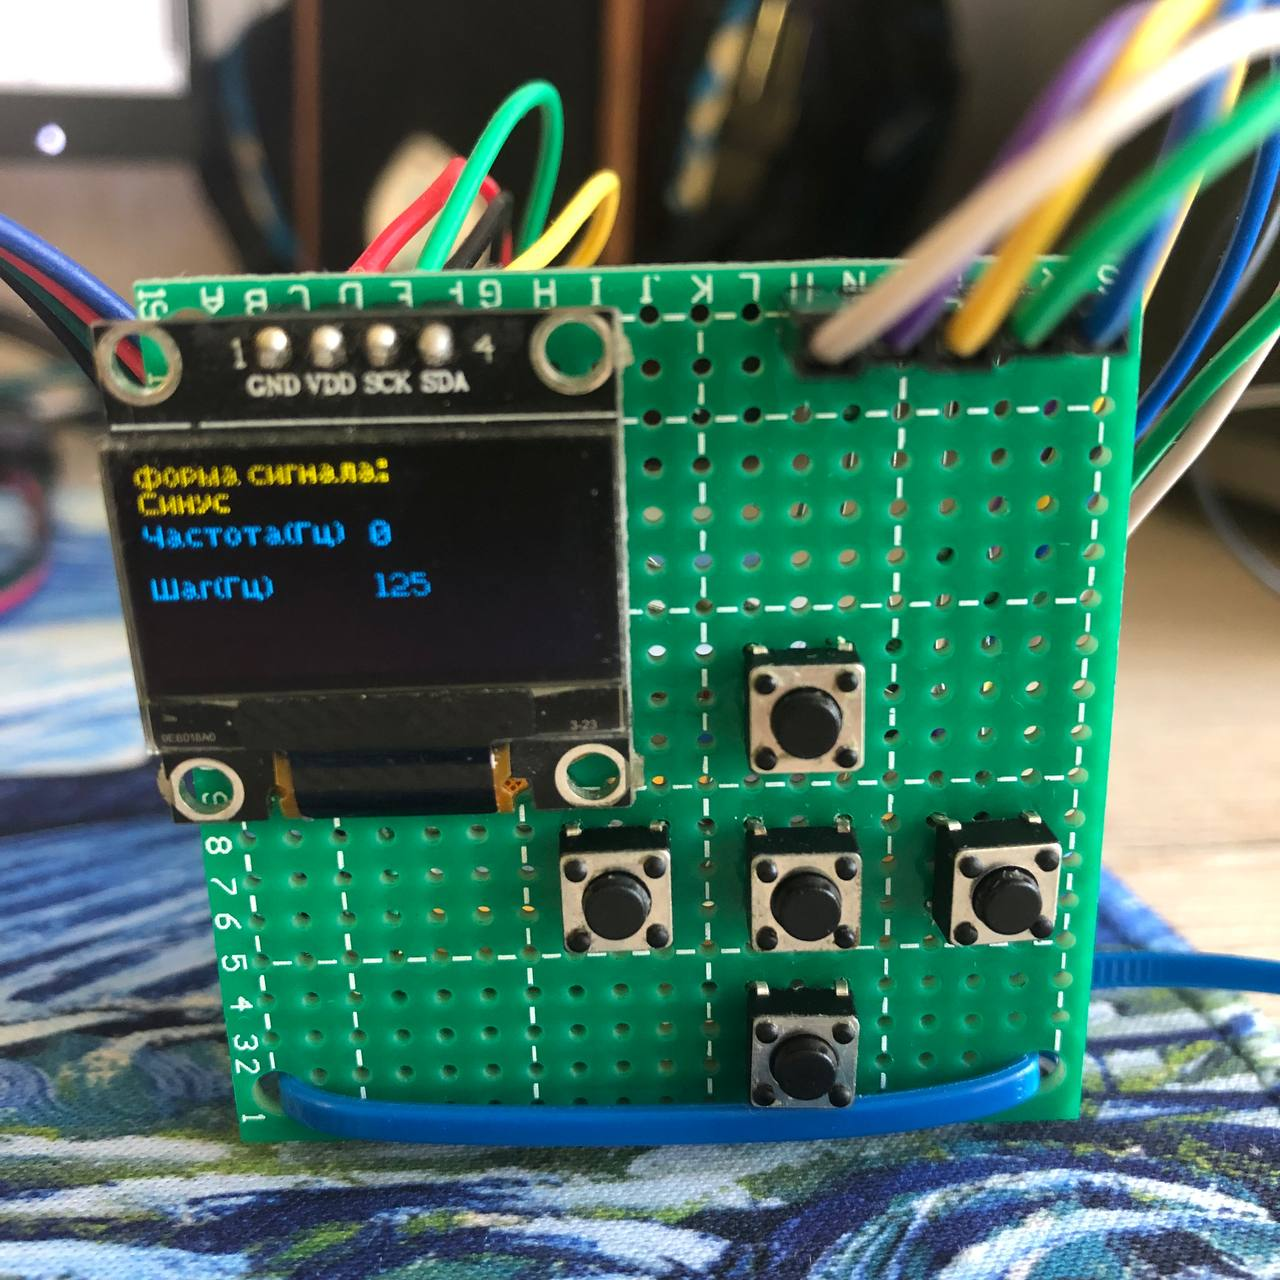
\includegraphics[width=0.8\textwidth]{../image/test1_u_st.jpg}
         \caption{Состояние устройства.}
     \end{subfigure}
     \hfill
     \begin{subfigure}[H]{0.5\textwidth}
         \centering
         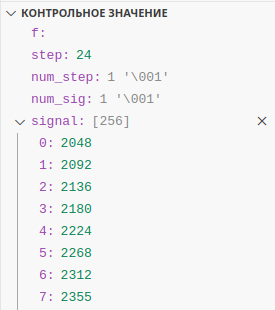
\includegraphics[width=0.725\textwidth]{../image/test1_o_st.png}
         \caption{Состояние в отладчике.}
     \end{subfigure}
        \caption{Процедура выбора шага частотой 125 Гц.}
	\end{figure}
	
	Выбор шага происходит циклично, поэтому для него требуется только одна кнопка. Самим же шагом по частоте является переменная step, которая содержит в себе для микроконтроллера код частоты, соответствующий частотам генерируемого сигнала.
	
	С помощью клавиш F- и F+ регулируется частота с заданным шагом. Возможный диапазон частот, который можно выставить 125 --- 50000 Гц. Алгоритм представлен блок-схемами (рис. 3.20).
	
	\begin{figure}[H]\captionsetup[subfigure]{font=normalsize}
     \begin{subfigure}[H]{1\textwidth}
         \centering
         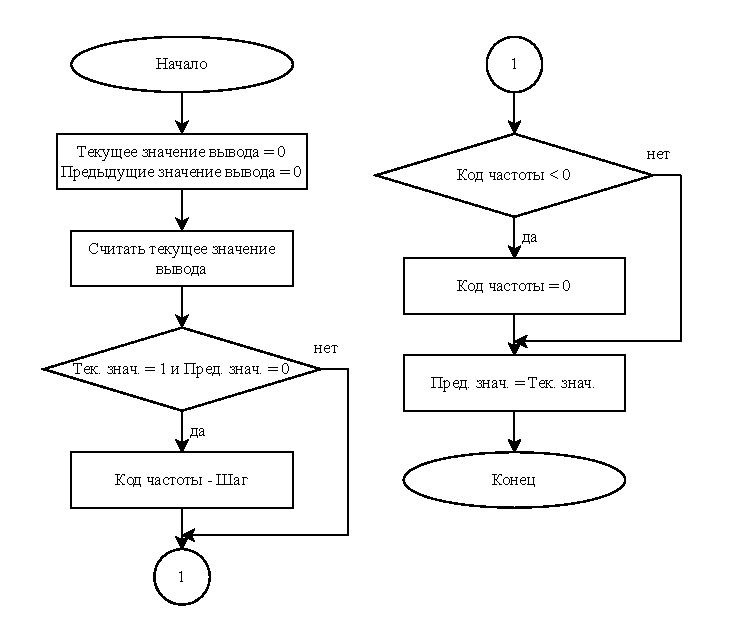
\includegraphics[width=0.775\textwidth]{../image/minus_freq.pdf}
         \caption{Блок-схема алгоритма уменьшения частоты.}
     \end{subfigure}
     \hfill
     \begin{subfigure}[H]{1\textwidth}
         \centering
         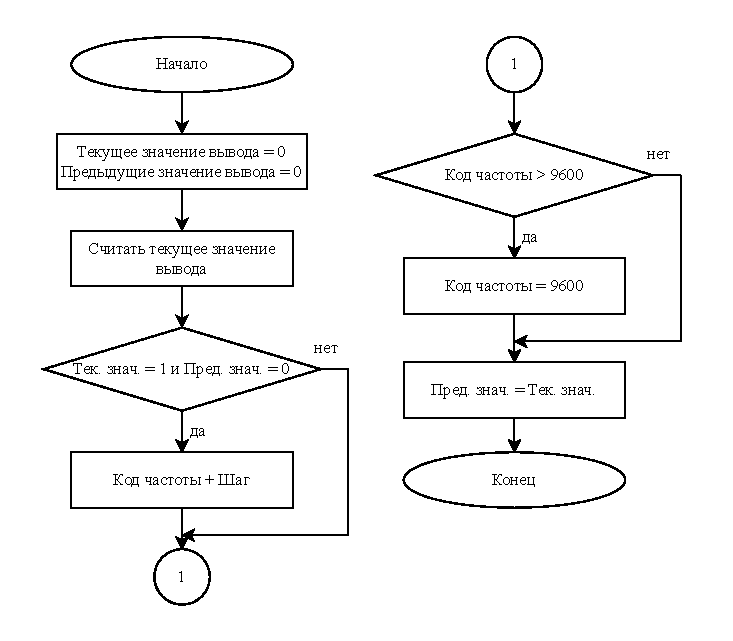
\includegraphics[width=0.775\textwidth]{../image/plus_freq.pdf}
         \caption{Блок-схема алгоритма увеличения частоты.}
     \end{subfigure}
        \caption{Блок-схемы алгоритмов регулировки частоты.}
	\end{figure}
	
	Все функции отрабатывают корректно. Выставим сигнал синуса с частотой 1875 Гц.
	
	\begin{figure}[H]\captionsetup[subfigure]{font=normalsize}
     \begin{subfigure}[H]{0.5\textwidth}
         \centering
         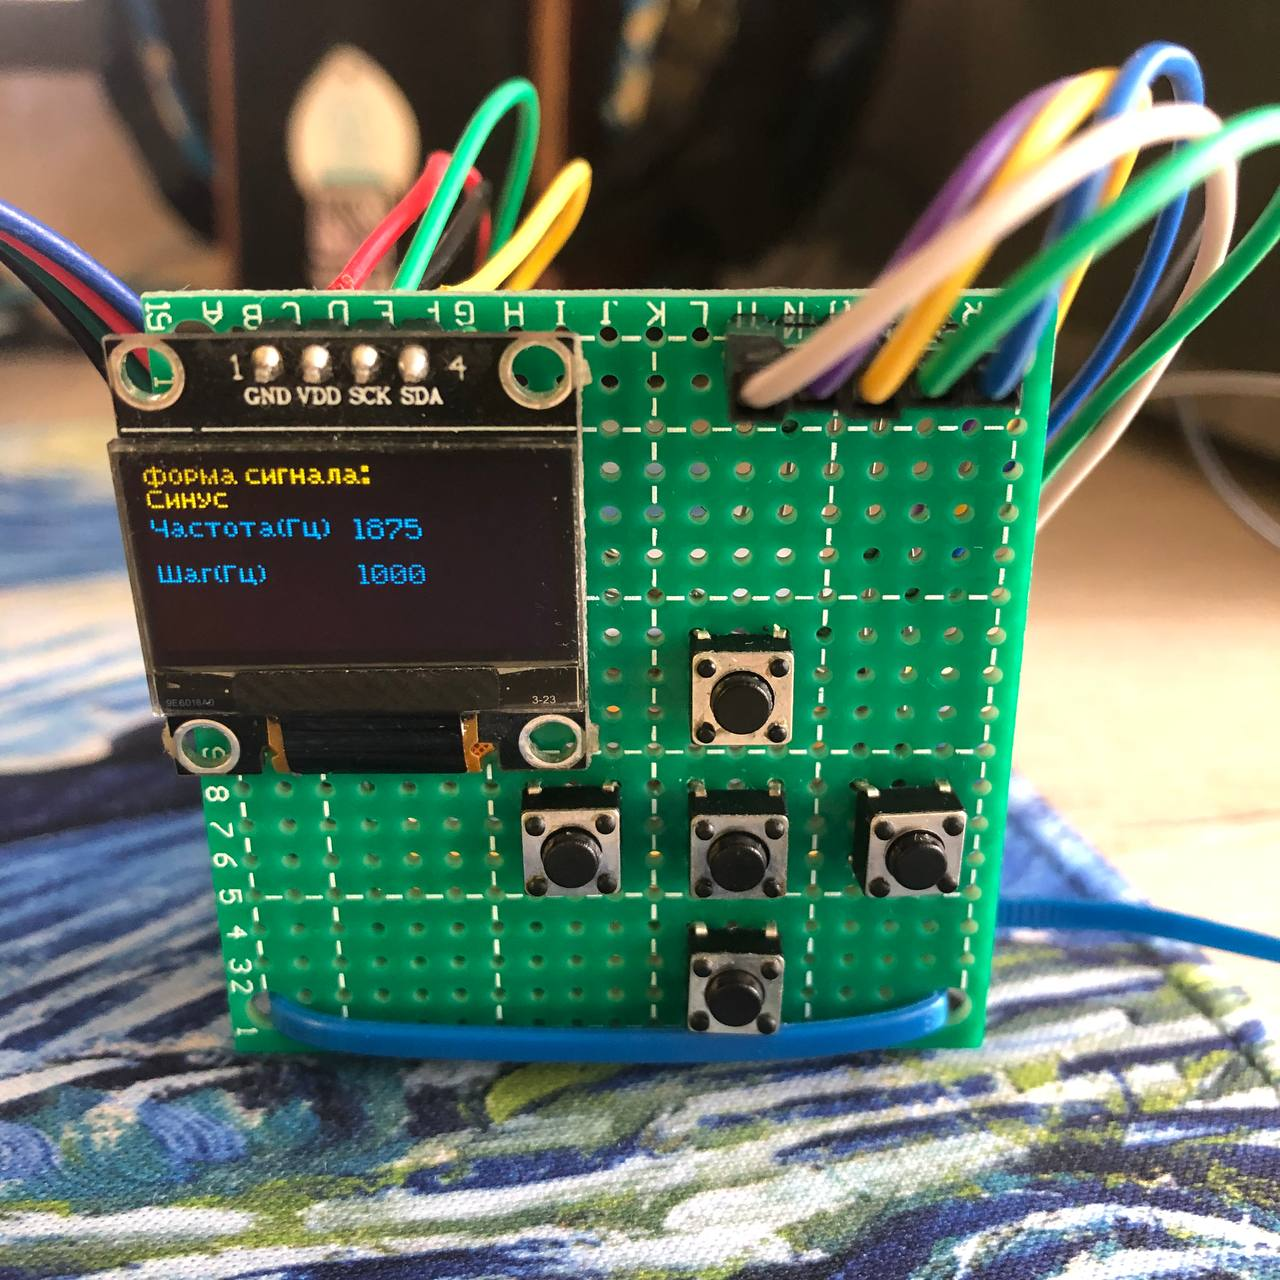
\includegraphics[width=0.7\textwidth]{../image/test4_u_f.jpg}
         \caption{Состояние устройства.}
    	\end{subfigure}
     \hfill
     \begin{subfigure}[H]{0.5\textwidth}
         \centering
         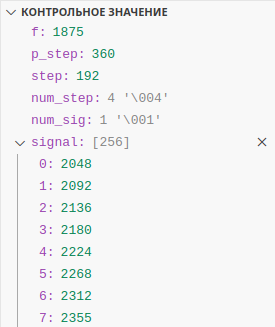
\includegraphics[width=0.62\textwidth]{../image/test4_o_f.png}
         \caption{Состояние в отладчике.}
     \end{subfigure}
        \caption{Выставленные параметры.}
	\end{figure}
	
	Снимем сигнал с осциллографа.
	\begin{figure}[H]
    \centering
    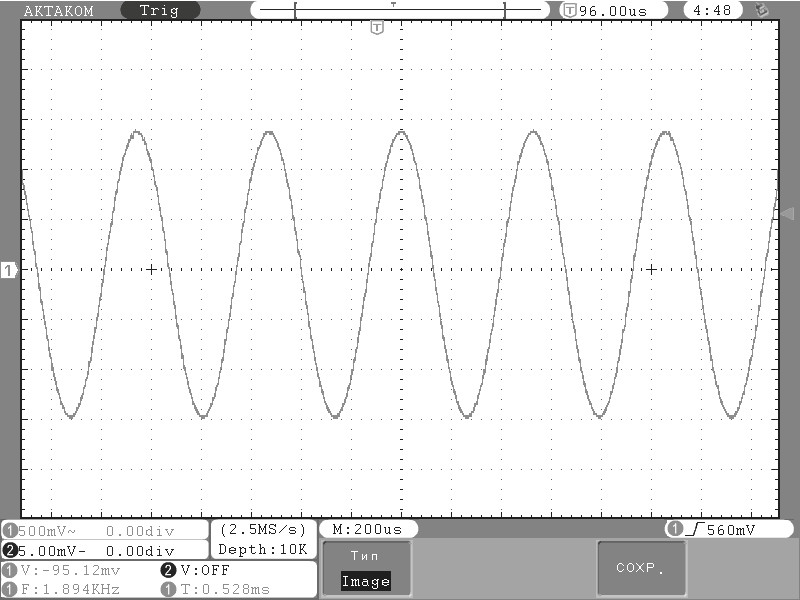
\includegraphics[width=0.75\textwidth]{../image/1875.bmp}
    \caption{Синусоидальный сигнал с частотой 1875 Гц.}
	\end{figure}	
	
	Рассмотрим все формы сигналов на частоте 1 кГц.
	
	На рис. 3.16 изображён синусоидальный сигнал с частотой 1 кГц.

	\begin{figure}[H]
    \centering
    \includegraphics[width=0.75\textwidth]{../image/sin1.bmp}
    \caption{Синусоидальный сигнал с частотой 1 кГц.}
	\end{figure}	


	На рис. 3.17 изображён прямоугольный сигнал с частотой 1 кГц.
	\begin{figure}[H]
    \centering
    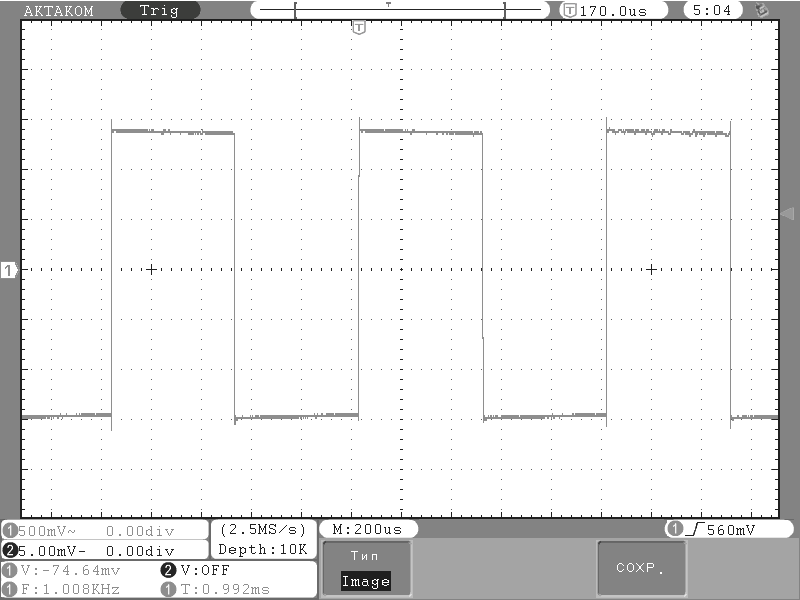
\includegraphics[width=0.75\textwidth]{../image/square1.bmp}
    \caption{Прямоугольный сигнал с частотой 1 кГц.}
	\end{figure}	
	
	На рис. 3.18 изображён треугольный сигнал с частотой 1 кГц.
	\begin{figure}[H]
    \centering
    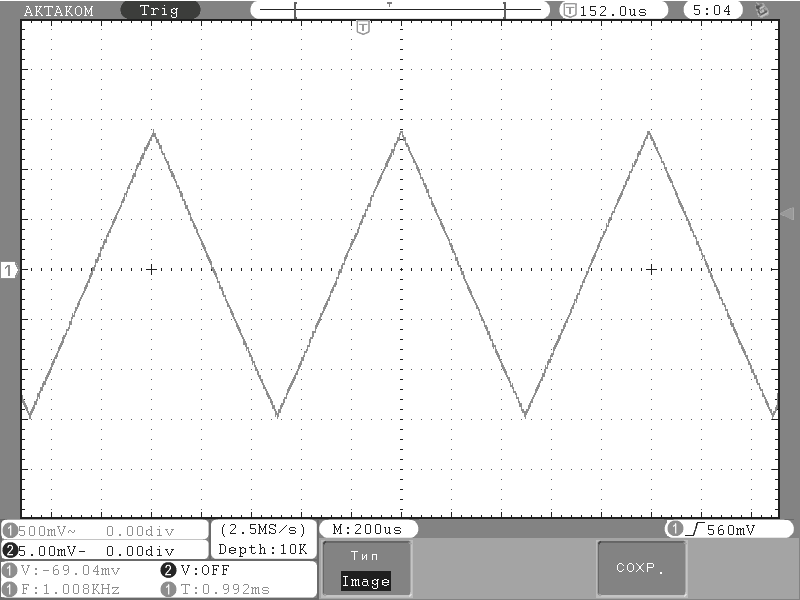
\includegraphics[width=0.75\textwidth]{../image/triangle1.bmp}
    \caption{Треугольный сигнал с частотой 1 кГц.}
	\end{figure}	

	На рис. 3.19 изображён обратный пилообразный сигнал с частотой 1 кГц.
	
	\begin{figure}[H]
    \centering
    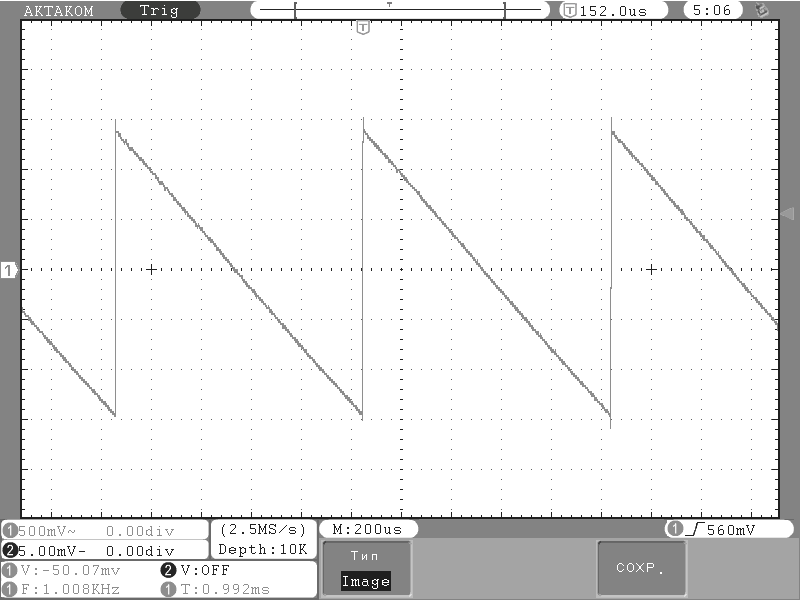
\includegraphics[width=0.75\textwidth]{../image/l_saw1.bmp}
    \caption{Обратный пилообразный сигнал с частотой 1 кГц.}
	\end{figure}	

	На рис. 3.20 изображён пилообразный сигнал с частотой 1 кГц.	
	\begin{figure}[H]
    \centering
    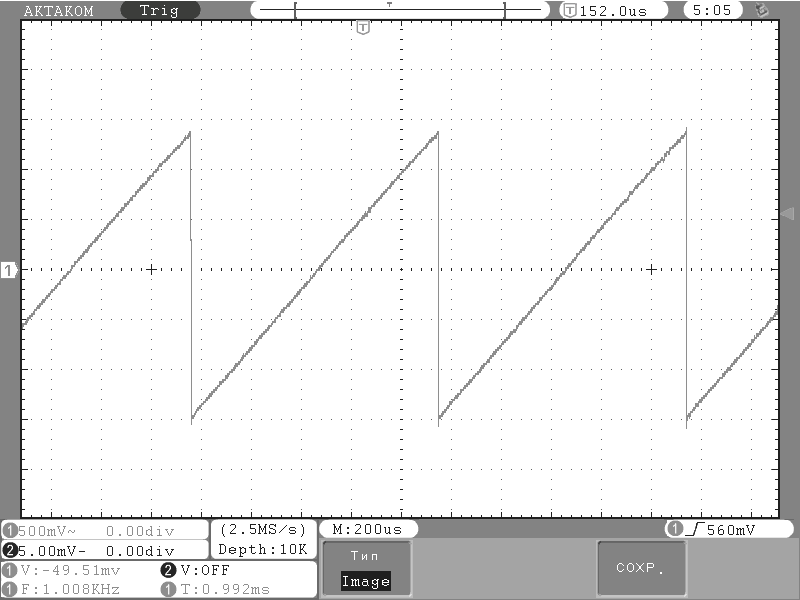
\includegraphics[width=0.75\textwidth]{../image/r_saw1.bmp}
    \caption{Пилообразный сигнал с частотой 1 кГц.}
	\end{figure}	
	
	Как можно заметить устройство генерирует все заданные формы сигналов. Рассмотрим более высокие частоты синуса (рис 3.21).
	
	\begin{figure}[H]
    \centering
    \includegraphics[width=0.75\textwidth]{../image/sin10.bmp}
    \caption{Синусоидальный сигнал с частотой 10 кГц.}
	\end{figure}	
	
	На 10 кГц уже можно наблюдать, что отсчёты сигнала не такие ровные. На 50 кГц синусоиду уже трудно узнать (рис. 3.22). На её период приходится 7 отсчётов.
	
	\begin{figure}[H]
    \centering
    \includegraphics[width=0.7\textwidth]{../image/sin50.bmp}
    \caption{Синусоидальный сигнал с частотой 50 кГц.}
	\end{figure}	
	
	Исходя из этого можно сделать вывод, что присутствует шум цифро-аналогового преобразователя. 
	
	Проведём анализ сигнала в программе GNU Octave~\cite{octave}. Возьмём записанные осциллографом отсчёты синусоидального сигнала на частоте 1 кГц и построим для сравнения такую же форму сигнала, но с заведомо большей частотой дискретизации. Будем считать построенную форму идеальным сигналом. Частота дискретизации ЦАП составляет 1 МГц, а для построения возьмём 5 МГц.
	
\begin{code}
\captionof{listing}{Сравнение сигналов}
\begin{minted}[mathescape,linenos,frame=lines,breaklines]{text}
clear all
sig = csvread('data.csv'); % сигнал с осциллографа
Td = sig(2,1)-sig(1,1); % период дискретизаци
t=linspace(0, 24999*Td, 25000); % интервал времени для идеального сигнала
f = 1000; % частота идеального сигнала
ideal_sin = -2.9 / 2 * sin(2 * pi * f * t) + 3.3 / 2 + 0.05; % идеальный сигнал
ideal_sin=ideal_sin.';
plot(t, sig(:,2), 'LineWidth', 0.5)
hold on;
plot(t, ideal_sin, 'LineWidth', 2)
xlabel('Время (с)');
ylabel('Напряжение (В)');
\end{minted}
\end{code}

	В итоге получим следующее изображение, из которого можно заметить, что сигнал с генератора не совпадает с идеальным, то есть его частота не составляет ровно 1 кГц (рис. 3.23.).
	
	\begin{figure}[H]
    \centering
    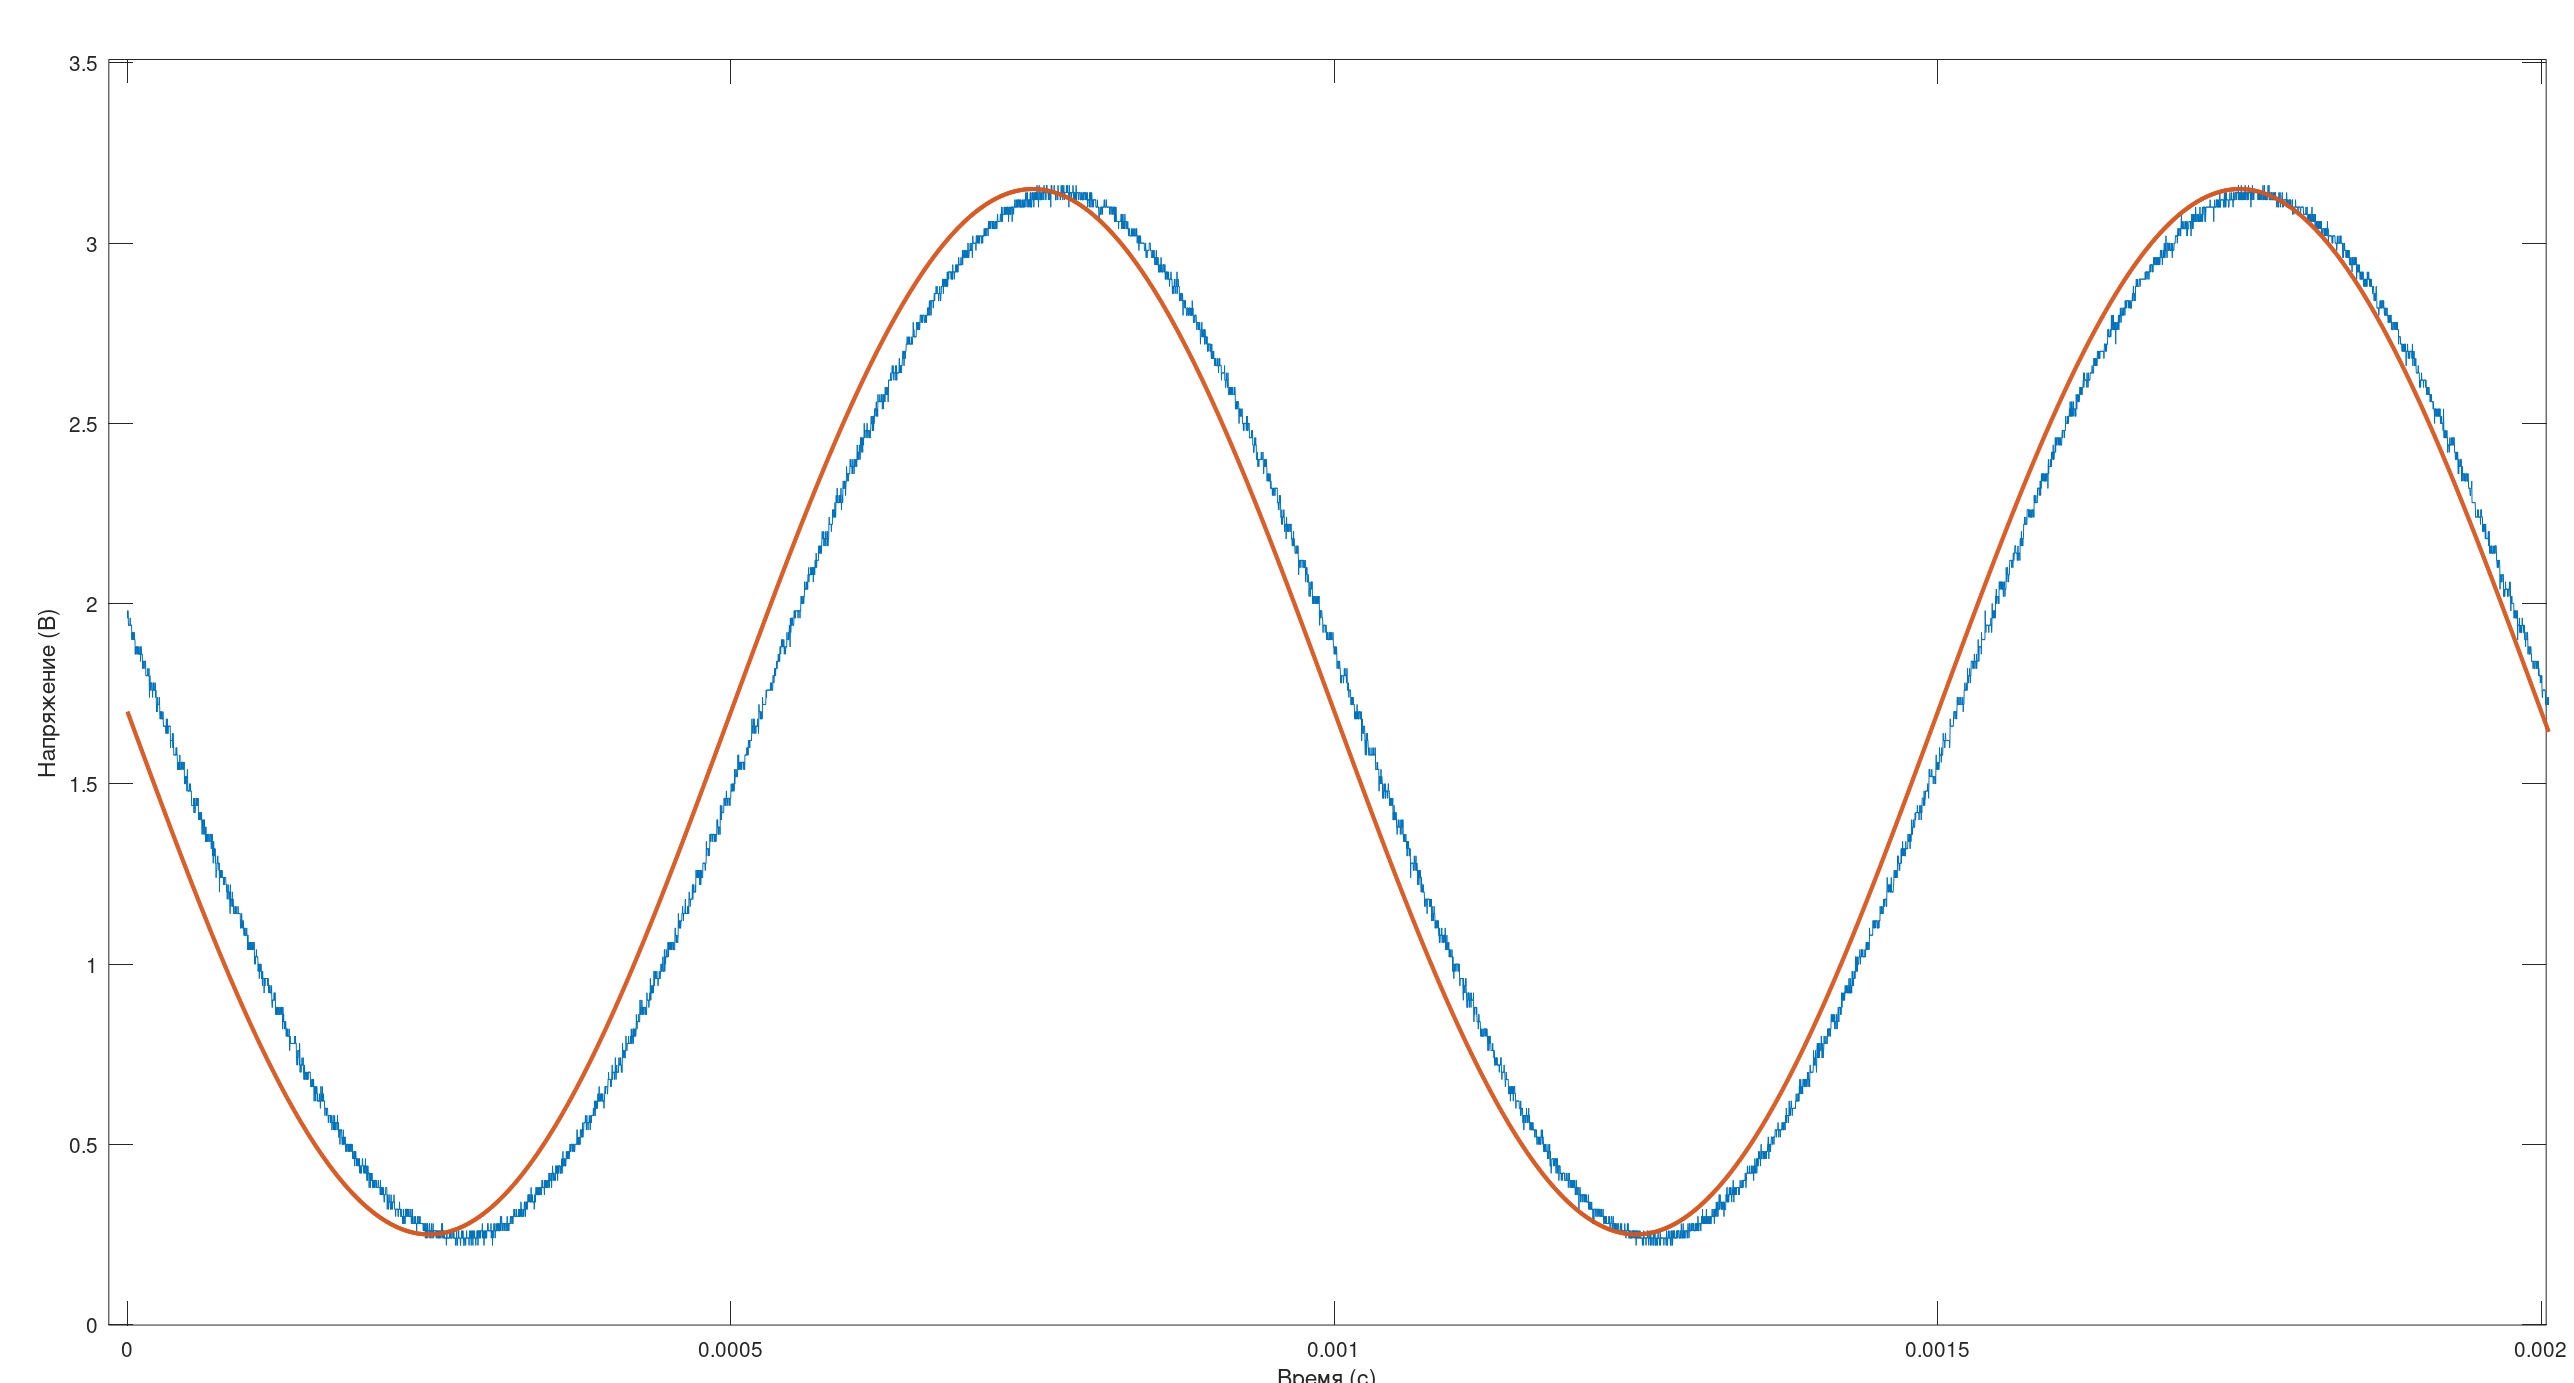
\includegraphics[width=1\textwidth]{../image/ideal.png}
    \caption{Сравнение записанного и идеального сигналов.}
	\end{figure}	
	
	Проведём спектральный анализ нашего сигнала, перейдя от временной составляющей к частотной с помощью быстрого преобразования Фурье~\cite{cos}.

\begin{code}
\captionof{listing}{Спектральный анализ}
\begin{minted}[mathescape,linenos,frame=lines,breaklines]{text}
fft_ideal = abs(fft(ideal_sin)/25000);
data_sig = sig(:, 2);
fft_sig = abs(fft(data_sig)/25000);
ff=linspace(0,24999/25000*1/Td, 1/Td/25000);
ff=ff.'

output_data_fft = zeros(length(fft_ideal), 2);
output_data_fft(:, 1) = fft_ideal;
output_data_fft(:, 2) = fft_sig;

csvwrite('fft.CSV', output_data_fft);
csvwrite('ff.CSV', ff);
\end{minted}
\end{code}
	
	На рис. 3.24 можно заметить смещение по частоте и утечку фазы.

	\begin{figure}[H]
    \centering
    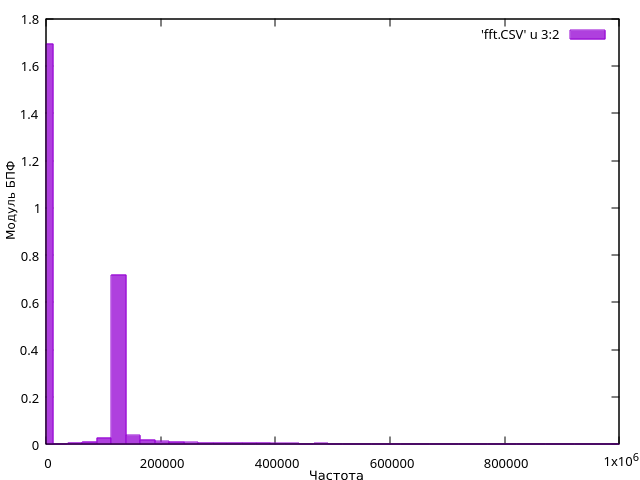
\includegraphics[width=1\textwidth]{../image/fft.png}
    \caption{Спектр сигнала.}
	\end{figure}	
	
		
	
\section{Вывод по третьей главе}
	Таким образом, генератор сигналов был реализован в виде макета. Тестирование показало, что устройство успешно выполняет заданные функции. Были проверены различные формы сигналов, а также возможность регулирования частоты с заданным шагом. Дополнительно был проведен анализ сигнала с помощью сравнения с построенным идеальным и рассмотрением спектра. 
	
	В качестве возможных усовершенствований можно рассмотреть:
	\begin{enumerate}
	\item Увеличение разрешения регулирования частоты и диапазона частот;
	\item Установка фильтра на выход цифро-аналогового преобразователя;
	\item Возможность регулировки амплитуды;
	\item Возможность регулировки фазы;
	\item Разработка печатной платы и корпуса.
	\end{enumerate}